\subsection{Packet Loss from 2022 to 2024} \label{sec:packet-loss}

We looked at the packet loss for the time range from 2022 to June 2024. We use
the Ping measurement from the RIPE Atlas built-in measurements, which by
default send three packets and collect the number of received packets.
Table~\ref{fig:packetloss-total} shows the resulting packet losses in percent
per country.

\begin{table}
	\footnotesize
	\caption{Packet Loss and Latency Correlation in 2022 to June 2024}
	\label{fig:packetloss-total}
	\begin{tabular}{rrlr}
		\toprule
		Sent      & Received  & Country                     & Packet
		Loss Ratio in \%                                             \\
		\midrule
		2150628   & 2134905   & Austria                     & 0.73   \\
		65021654  & 62438854  & Australia                   & 3.97   \\
		22727113  & 22211676  & Belgium                     & 2.27   \\
		1176124   & 1168114   & Benin                       & 0.68   \\
		124263104 & 121160149 & Canada                      & 2.50   \\
		2843      & 2832      & Switzerland                 & 0.39   \\
		3626230   & 3617474   & Chile                       & 0.24   \\
		8092876   & 8074360   & Czechia                     & 0.23   \\
		96089885  & 85983781  & Germany                     & 10.52  \\
		21714610  & 21001677  & Spain                       & 3.28   \\
		432934    & 418925    & Falkland Islands (Malvinas) & 3.24   \\
		321919833 & 299847062 & France                      & 6.86   \\
		83840509  & 80720387  & United Kingdom              & 3.72   \\
		12522224  & 12318835  & Greece                      & 1.62   \\
		271185    & 265100    & Guam                        & 2.24   \\
		18472787  & 18217243  & Haiti                       & 1.38   \\
		37188354  & 35583136  & Italy                       & 4.32   \\
		4160290   & 3829356   & Kiribati                    & 7.95   \\
		127756    & 121937    & Madagascar                  & 4.55   \\
		20450037  & 17548642  & Netherlands                 & 14.19  \\
		26654399  & 21785387  & Philippines                 & 18.27  \\
		18739794  & 18670207  & Poland                      & 0.37   \\
		7047181   & 6967111   & Réunion                     & 1.14   \\
		9975257   & 9922734   & Sweden                      & 0.53   \\
		578852548 & 557475491 & United States               & 3.69   \\
		18571694  & 18463935  & Virgin Islands, U.S.        & 0.58   \\
		\bottomrule
	\end{tabular}
\end{table}

The results are surprising as some countries experience very high packet
losses, while other neighboring countries have rather low packet loss ratios.
For example, Germany and Netherlands are well-developed countries with a
relatively high number of \ac{GS}es. One would expect a low packet loss, which
is not the case. Both countries hold packet loss ratios above ten percent. On
the other hand, neighboring countries like Austria do not show such a pattern.
Another country with remarkably high packet loss are the Philippines, which
have the highest packet loss ratio of all countries.

Overall, most countries experience packet loss ratios at one to four percent,
with some having an even lower value. The lowest value has Czechia with
0.23~\%, while Chile has 0.24~\%.

However, the time range is quite long. Therefore, we looked at the time range
in a more fine-grained interval for the above-mentioned countries.
Figure~\ref{fig:packet-loss-fine-grained} show the packet loss ratios for each
month from January 2022 to June 2024 for Germany, the Netherlands, the
Philippines, and the USA. The first three were chosen as they are noticeable in
Table~\ref{fig:packetloss-total}. The USA was chosen, as it holds the most data
and is therefore a good comparison.

\begin{figure}
	\centering
	\begin{subfigure}[t]{0.47\linewidth}
		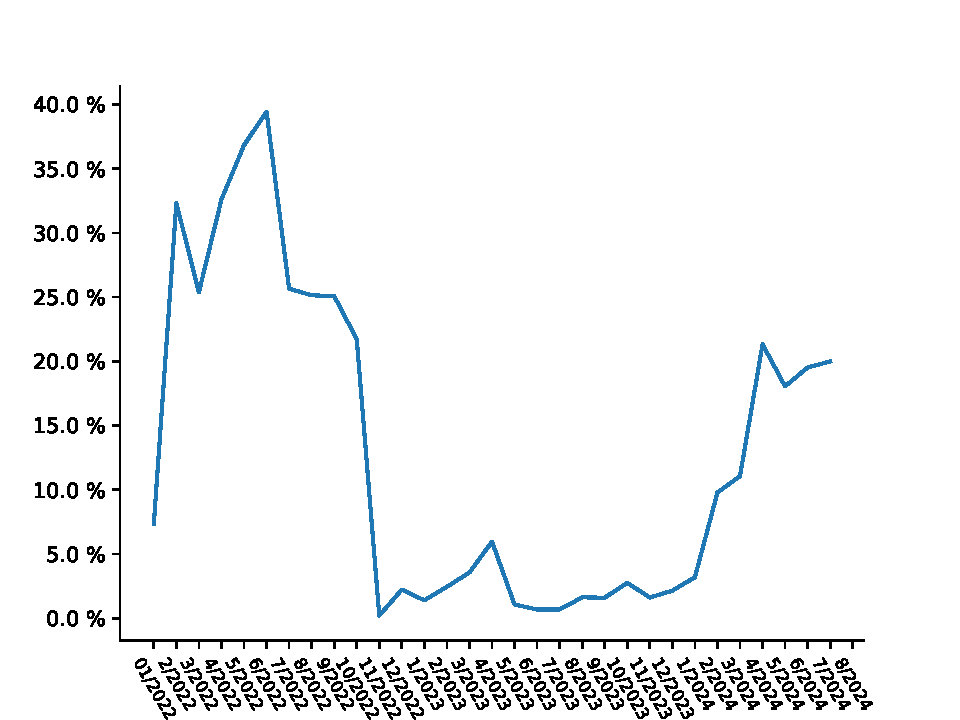
\includegraphics[width=\linewidth]{./chapters/4-results/packet-loss/img/DE.pdf}
		\caption{Germany}
	\end{subfigure}
	\begin{subfigure}[t]{0.47\linewidth}
		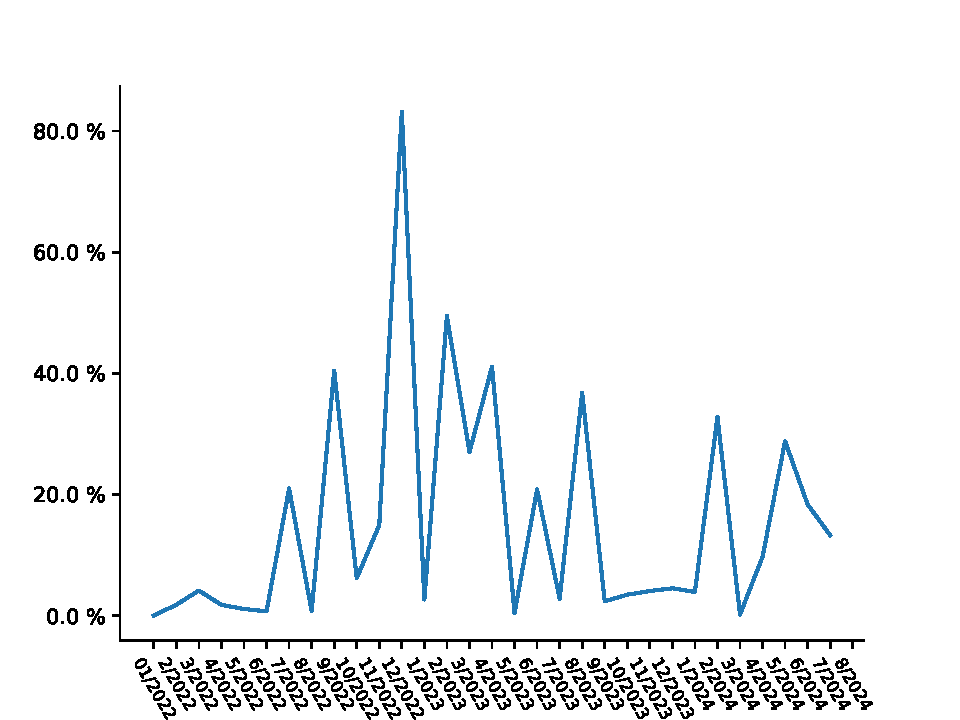
\includegraphics[width=\linewidth]{./chapters/4-results/packet-loss/img/NL.pdf}
		\caption{Netherlands}
	\end{subfigure}
	\begin{subfigure}[t]{0.47\linewidth}
		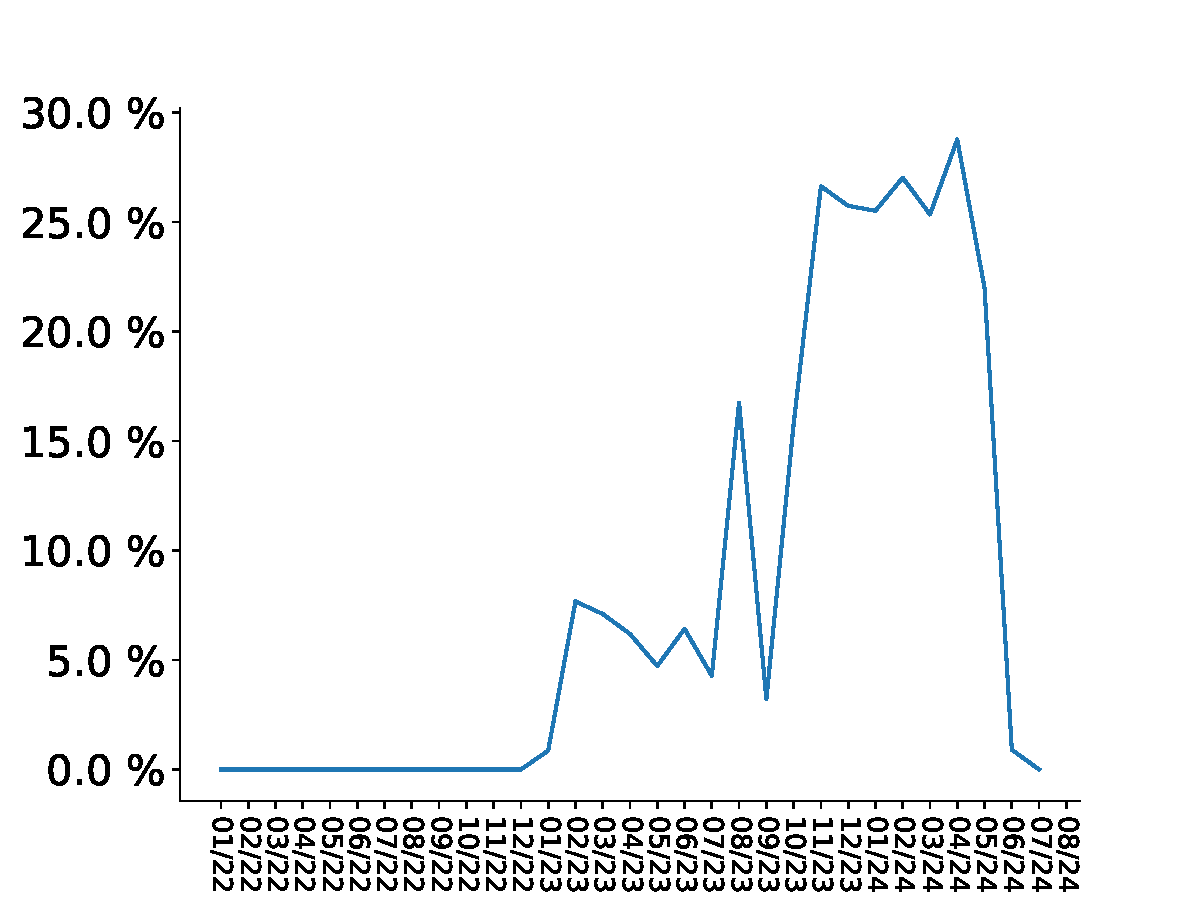
\includegraphics[width=\linewidth]{./chapters/4-results/packet-loss/img/PH.pdf}
		\caption{Philippines}
	\end{subfigure}
	\begin{subfigure}[t]{0.47\linewidth}
		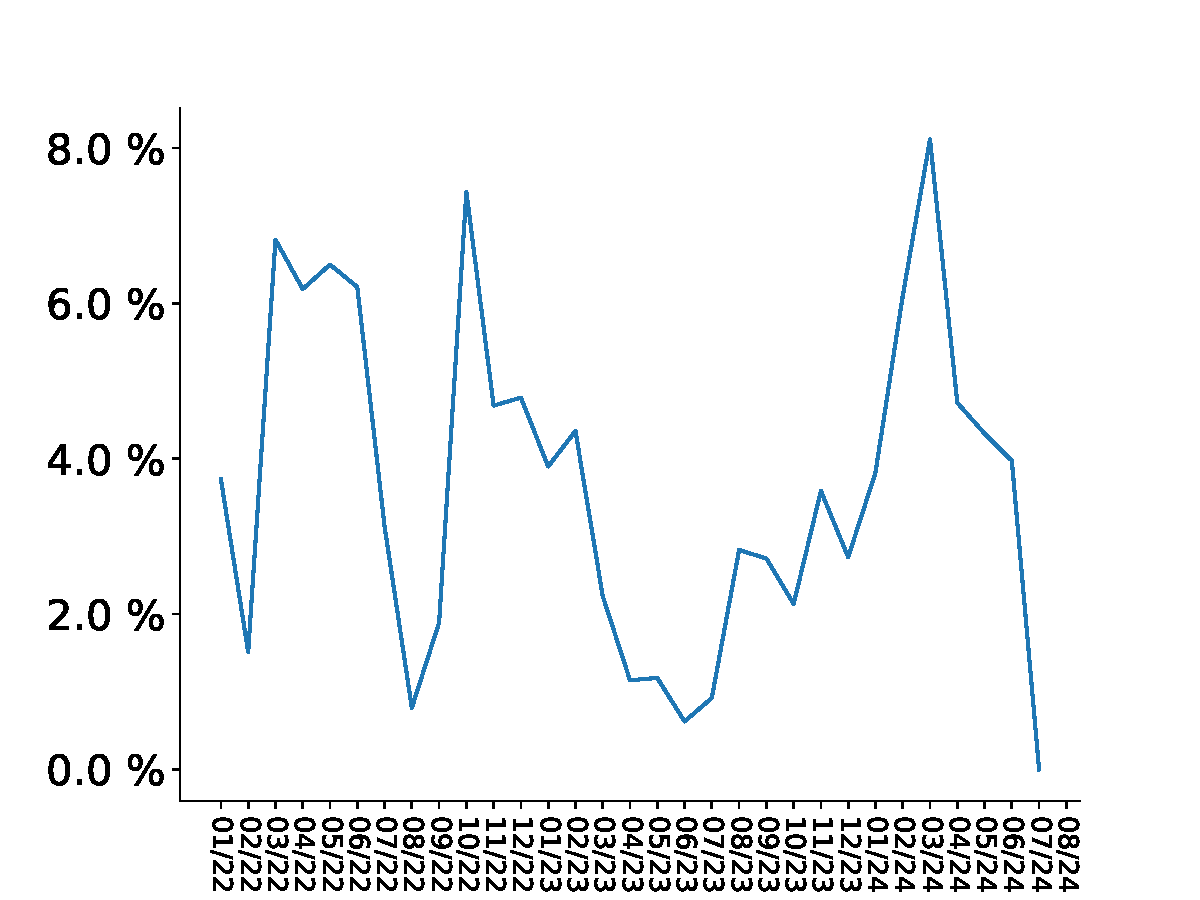
\includegraphics[width=\linewidth]{./chapters/4-results/packet-loss/img/US.pdf}
		\caption{USA}
	\end{subfigure}
	\caption{Packet Loss Ratios in Percent in individual Month from January
		2022 to June 2024}
	\label{fig:packet-loss-fine-grained}
\end{figure}

One can see that Germany experienced high volumes of packet loss in 2022
reaching as high as 40~\% packet loss in June 2022. This was followed by a
period of little packet loss ratios in 2023. Likely, papers taking measurements
at this time will report Germany to have very little packet loss. In 2024, the
trend is going back towards higher packet losses.

The Netherlands show fluctuating pattern that even reaches values of 80~\%
packet loss in December~2022. However, little conclusions can be made except
for the assumption that the connection is highly instable.

The Philippines only hold data since 2023. Therefore, we cannot make
conclusions about the packet loss in the Philippines in 2022. In 2023 however,
the packet loss was around five to eight percent, until in August 2023, the
packet loss rose to more than fifteen percent. In 2024, the packet loss even
rose above twenty-five percent. June 2024 saw a sudden reduction in packet
loss. However, there is to little time series data to determine whether this is
an outlier.

The USA shows a similar pattern to Germany. In 2022, the packet loss was
relatively high, followed by a reducion in 2023, followed by an increase in
2024. However, there are two key differences when comparing Germany and the
USA: (1) the USA experiences lower percentages in packet loss and (2) a
reduction of packet loss is suggested starting in April 2024, which does not
happen for Germany.

\begin{takeaway}{Packet Loss in Starlink}
	The packet loss of Starlink connections is for most countries in the
	range of 1~--~4 \%. However, there are major differences and regional
	proximity does not seem to play a role. Additionally, 2023 has
	experienced better packet loss results compared to 2022 and 2024. This
	is a key difference to the latency analysis, where 2023 has experienced
	the worst results. It seems that Starlink can only op optimize for
	either packet loss and latency. It is in question, whether both values
	correlate.
\end{takeaway}

